  \documentclass[12pt,a4paper]{article}

  \usepackage[utf8]{inputenc}
  \usepackage[T1]{fontenc}
  \usepackage[spanish,es-nodecimaldot,es-noquoting]{babel}
  \usepackage{graphicx}
  \usepackage{geometry}
  \geometry{top=2.5cm,bottom=2.5cm,left=2.5cm,right=2.5cm,headheight=15pt}
  \usepackage{xcolor}
  \usepackage{hyperref}
  \usepackage{longtable}
  \usepackage{tabularx}
  \usepackage{booktabs}
  \usepackage{listings}
  \usepackage{fancyhdr}
  \usepackage{tcolorbox}
  \usepackage{titlesec}
  \usepackage{enumitem}
  \usepackage{caption}
  \usepackage{amsmath}
  \usepackage{float}

  % Colores institucionales y de código
  \definecolor{unsaacblue}{RGB}{0, 51, 102}
  \definecolor{darkblue}{RGB}{10, 40, 95}
  \definecolor{accentblue}{RGB}{25, 118, 210}
  \definecolor{codegreen}{RGB}{46, 125, 50}
  \definecolor{codegray}{RGB}{100, 116, 139}
  \definecolor{codepurple}{RGB}{124, 58, 237}
  \definecolor{backcolour}{RGB}{248, 250, 252}
  \definecolor{bordercolor}{RGB}{226, 232, 240}
  \definecolor{calloutbg}{RGB}{240, 249, 255}
  \definecolor{calloutborder}{RGB}{56, 189, 248}

  % Configuración de listings para código Dart / Flutter
  \lstdefinelanguage{Dart}{
    morekeywords={
      abstract,as,assert,async,await,break,case,catch,class,const,continue,
      default,deferred,do,dynamic,else,enum,export,extends,external,factory,
      false,final,finally,for,Function,get,hide,if,implements,import,in,
      interface,is,late,library,mixin,new,null,of,on,operator,part,rethrow,
      return,set,show,static,super,switch,sync,this,throw,true,try,typedef,
      var,void,while,with,yield,override,required
    },
    morecomment=[l]{//},
    morecomment=[s]{/*}{*/},
    morestring=[b]',
    morestring=[b]",
    sensitive=true
  }

  \lstset{
    language=Dart,
    backgroundcolor=\color{backcolour},
    commentstyle=\color{codegreen}\itshape,
    keywordstyle=\color{unsaacblue}\bfseries,
    numberstyle=\tiny\color{codegray},
    stringstyle=\color{codepurple},
    basicstyle=\ttfamily\footnotesize,
    breakatwhitespace=false,
    breaklines=true,
    captionpos=b,
    keepspaces=true,
    numbers=left,
    numbersep=7pt,
    showspaces=false,
    showstringspaces=false,
    showtabs=false,
    tabsize=2,
    frame=single,
    rulecolor=\color{bordercolor},
    xleftmargin=15pt,
    framexleftmargin=15pt
  }

  \hypersetup{
    colorlinks=true,
    linkcolor=unsaacblue,
    filecolor=magenta,
    urlcolor=accentblue,
    citecolor=unsaacblue
  }

  % Encabezados y pies de página
  \pagestyle{fancy}
  \fancyhf{}
  \fancyhead[L]{\small\color{codegray}UNSAAC - Desarrollo de Software II}
  \fancyhead[R]{\small\color{codegray}Práctica 05: Eventos e Interactividad en Flutter}
  \fancyfoot[C]{\thepage}
  \renewcommand{\headrulewidth}{0.4pt}
  \renewcommand{\footrulewidth}{0.4pt}

  \begin{document}

  % ==============================================================================
  % CARÁTULA OFICIAL INSTITUCIONAL UNSAAC
  % ==============================================================================
  \begin{titlepage}
      \centering
      {\bfseries\large UNIVERSIDAD NACIONAL DE SAN ANTONIO ABAD DEL CUSCO\par}
      \vspace{0.2cm}
      {\bfseries\normalsize FACULTAD DE INGENIERÍA ELÉCTRICA, ELECTRÓNICA, INFORMÁTICA Y MECÁNICA\par}
      \vspace{0.2cm}
      {\bfseries\normalsize ESCUELA PROFESIONAL DE INGENIERÍA INFORMÁTICA Y DE SISTEMAS\par}
      \vspace{0.8cm}
      
\includegraphics[width=0.35\textwidth]{unsaac.jpg}\par
      \vspace{0.8cm}
      {\Large\bfseries ASIGNATURA: DESARROLLO DE SOFTWARE II\par}
      \vspace{0.4cm}
      {\large\bfseries TRABAJO: PRÁCTICA 05: MANEJO DE EVENTOS E INTERACTIVIDAD EN FLUTTER\par}
      \vspace{0.4cm}
      {\large\bfseries IMPLEMENTACIÓN INTEGRAL DE EVENTOS, ENTRADAS DE USUARIO, GESTIÓN REACTIVA DE ESTADO Y SUITE DE EJERCICIOS (BÁSICO, INTERMEDIO Y AVANZADO)\par}
      \vspace{1.2cm}
      \begin{flushleft}
      \textbf{DOCENTE RESPONSABLE:} \\
      Ing. Hans Harley Ccacyahuillca Bejar\\[0.5cm]
      \textbf{AUTOR / DESARROLLADOR:} \\
      SUPA CUSIPAUCAR, Yeferson - 220553\\[0.5cm]
      \textbf{SEMESTRE ACADÉMICO:} \\
      2026-II (Décimo Semestre)\\[0.5cm]
      \textbf{REPOSITORIO OFICIAL:} \\
      \url{https://github.com/YefersonSupa/Desarrollo_SoftwareII}
      \end{flushleft}
      \vfill
      {\bfseries\large Cusco - Perú\par}
      {\bfseries 2026\par}
  \end{titlepage}

  \tableofcontents
  \newpage

  % ==============================================================================
  % 1. INFORMACIÓN GENERAL Y FICHA TÉCNICA
  % ==============================================================================
  \section{Información General del Proyecto}

  El presente informe técnico documenta el diseño, desarrollo, verificación y ejecución de la \textbf{Práctica de Laboratorio N$^\circ$ 5: Manejo de Eventos e Interactividad en Flutter} para la asignatura de \textbf{Desarrollo de Software II}. En esta entrega se implementa una aplicación móvil reactiva y desacoplada construida sobre \textbf{Flutter 3.47.4} y \textbf{Dart 3.13.3}, denominada \texttt{events\_app}.

  La aplicación resuelve de forma exhaustiva los \textbf{4 ejemplos fundamentales} de la guía oficial de cátedra y los \textbf{9 ejercicios propuestos} distribuidos en tres niveles de complejidad ascendente (Básico, Intermedio y Avanzado), adicionando una consola de auditoría de eventos en vivo que inspecciona en tiempo real el flujo de gestos y mutaciones de estado de la interfaz de usuario.

  \begin{tcolorbox}[colback=calloutbg,colframe=calloutborder,title=\textbf{Ficha Técnica de la Práctica 05}]
  \textbf{Institución:} Universidad Nacional de San Antonio Abad del Cusco (UNSAAC)\\
  \textbf{Facultad:} Ingeniería Eléctrica, Electrónica, Informática y Mecánica\\
  \textbf{Escuela Profesional:} Ingeniería Informática y de Sistemas\\
  \textbf{Asignatura:} Desarrollo de Software II\\
  \textbf{Docente Responsable:} Ing. Hans Harley Ccacyahuillca Bejar\\
  \textbf{Estudiante:} SUPA CUSIPAUCAR, Yeferson (Código: 220553)\\
  \textbf{Entorno de Desarrollo:} Flutter SDK 3.47.4, Dart SDK 3.13.3, Material 3\\
  \textbf{Ubicación del Código Fuente:} \texttt{/lab\_05/events\_app}\\
  \textbf{Repositorio en GitHub:} \url{https://github.com/YefersonSupa/Desarrollo_SoftwareII}
  \end{tcolorbox}

  % ==============================================================================
  % 2. FUNDAMENTOS DE LA ARQUITECTURA DE EVENTOS E INTERACTIVIDAD EN FLUTTER
  % ==============================================================================
  \section{Fundamentos de la Arquitectura de Eventos e Interactividad}

  \subsection{El Paradigma Declarativo y Reactivo de Flutter}
  En el modelo declarativo de Flutter, la interfaz gráfica no es modificada imperativamente manipulando nodos DOM o instancias de vistas mutables, sino que se formula como una función pura del estado:
  \begin{equation}
  UI = f(State)
  \end{equation}
  Cuando el usuario interactúa con la aplicación (presiona un botón, escribe en un campo de texto o realiza un doble toque), se dispara un evento. El controlador del evento actualiza el estado interno y solicita al framework redibujar la interfaz mediante la notificación de recreación del subárbol correspondiente.

  \subsection{Diferenciación entre StatelessWidget y StatefulWidget}
  Flutter organiza sus widgets en dos grandes familias según la variabilidad de su configuración en el tiempo:
  \begin{enumerate}[leftmargin=*]
      \item \textbf{StatelessWidget:} Widgets inmutables cuya apariencia depende únicamente de los parámetros suministrados en su constructor. No mantienen un ciclo de vida interno ni variables mutables.
      \item \textbf{StatefulWidget:} Widgets cuya configuración genera un objeto persistente de tipo \texttt{State<T>}. El objeto \texttt{State} reside en el \textit{Element Tree} y conserva sus variables a lo largo de las reconstrucciones sucesivas de la UI.
  \end{enumerate}

  \subsection{El Mecanismo de Mutación con setState()}
  El método \texttt{setState(VoidCallback fn)} es el motor de reactividad nativo en Flutter. Su ejecución cumple tres etapas secuenciales fundamentales:
  \begin{enumerate}[leftmargin=*]
      \item Ejecuta síncronamente la función de callback \texttt{fn()}, modificando las variables internas de estado.
      \item Marca al elemento asociado (\texttt{StatefulElement}) con la bandera interna \textit{dirty} (sucio o desactualizado).
      \item Agenda una fase de construcción (\textit{scheduleBuildFor}) para el siguiente ciclo del renderizador (\textit{frame}), invocando nuevamente el método \texttt{build(BuildContext context)} de forma eficiente.
  \end{enumerate}

  \begin{lstlisting}[caption={Estructura canónica del uso de setState en Flutter}]
  void _incrementarContador() {
    setState(() {
      _contador++; // Modificacion sincronica de la variable de estado
    }); // Notificacion automatica al Element Tree para redibujar
  }
  \end{lstlisting}

  \subsection{Detección y Reconocimiento de Gestos con GestureDetector}
  Flutter procesa las interacciones de puntero a través de la capa de bajo nivel \texttt{GestureBinding}, la cual recibe paquetes táctiles como \texttt{PointerDownEvent}, \texttt{PointerMoveEvent} y \texttt{PointerUpEvent}. El widget de alto nivel \texttt{GestureDetector} actúa como un concentrador de gestores de reconocimiento (\textit{GestureRecognizers}) resolviendo gestos semánticos complejos mediante un proceso denominado \textit{Gesture Arena} (arena de gestos):
  \begin{itemize}[leftmargin=*]
      \item \texttt{onTap}: Toque simple sin desplazamiento significativo.
      \item \texttt{onDoubleTap}: Detección de dos toques consecutivos en una misma coordenada espacial dentro de una ventana temporal acotada ($\approx 300-400$\,ms).
      \item \texttt{onLongPress}: Pulsación continua sostenida por más de $500$\,ms.
      \item \texttt{onPanUpdate} / \texttt{onHorizontalDragUpdate}: Seguimiento de arrastre vectorial bidimensional.
  \end{itemize}

  % ==============================================================================
  % 3. DESARROLLO DE LOS EJEMPLOS Y MINI PROYECTO DE LA GUÍA OFICIAL
  % ==============================================================================
  \section{Desarrollo de los Ejemplos y Mini Proyecto de la Guía Oficial}

  En el módulo interactivo \texttt{GuideExamplesScreen}, se materializaron los cuatro componentes de demostración pedagógica de la guía:

  \subsection{Ejemplo 1: Botón Interactivo (Contador con FloatingActionButton)}
  Demuestra la creación de un \texttt{StatefulWidget} que vincula un botón de acción flotante con una variable entera \texttt{contador}. Cada pulsación ejecuta \texttt{setState()}, reflejando el incremento numérico en un widget \texttt{Text} central y emitiendo una notificación al bus de auditoría.

  \subsection{Ejemplo 2: Entrada de Texto en Tiempo Real}
  Implementa un campo de captura de datos mediante \texttt{TextField} y un controlador persistente \texttt{TextEditingController}. Utiliza el callback \texttt{onChanged: (texto) \{ ... \}} para actualizar reactivamente una tarjeta de vista previa e imprimir en consola el flujo continuo de caracteres tecleados por el usuario.

  \subsection{Ejemplo 3: Manejo de Múltiples Gestos Táctiles}
  Aplica un contenedor interactivo envuelto por un \texttt{GestureDetector}. Dependiendo del estímulo aplicado por el operador:
  \begin{itemize}[leftmargin=*]
      \item Un solo toque (\texttt{onTap}): Muta la caja a color azul y suma 1 punto.
      \item Doble toque (\texttt{onDoubleTap}): Muta la caja a color púrpura y suma 2 puntos.
      \item Pulsación sostenida (\texttt{onLongPress}): Muta la caja a color naranja intenso y suma 5 puntos.
  \end{itemize}

  \subsection{Mini Proyecto: Formulario Interactivo con Saludo Dinámico}
  Combina el campo de entrada de texto con una tarjeta reactiva decorada con un gradiente institucional azul UNSAAC. A medida que el usuario escribe su nombre en el \texttt{TextField}, la interfaz transmuta en vivo el mensaje de bienvenida generando la cadena \texttt{Hola, \$nombre}, incorporando validaciones visuales cuando el campo se encuentra vacío (\textit{Hola, invitado}).

  % ==============================================================================
  % 4. IMPLEMENTACIÓN Y ANÁLISIS DE LOS 9 EJERCICIOS PROPUESTOS
  % ==============================================================================
  \section{Implementación y Análisis de los Ejercicios Propuestos}

  Los 9 ejercicios propuestos en la guía se organizaron rigurosamente por niveles de dificultad, dotando a cada uno de componentes gráficos avanzados y manejo estricto de eventos.

  \subsection{Nivel Básico}

  \subsubsection{Ejercicio 1: Botón que Modifica el Color de Fondo}
  \textbf{Objetivo:} Alterar dinámicamente el color de fondo de un contenedor ante la pulsación de un botón interactivo.\\
  \textbf{Implementación Técnica:}
  Se implementó un \texttt{AnimatedContainer} con interpolación suave (\texttt{duration: 400ms, curve: Curves.easeInOut}). Se suministró un botón principal que genera valores cromáticos aleatorios en formato RGB mediante la clase \texttt{Random}:
  \begin{lstlisting}[caption={Generación de color aleatorio y mutación de estado}]
  void _changeToRandomColor() {
    final random = Random();
    final newColor = Color.fromARGB(
      255,
      random.nextInt(220) + 20,
      random.nextInt(220) + 20,
      random.nextInt(220) + 20,
    );
    setState(() {
      _backgroundColor = newColor;
      _colorHistory.insert(0, newColor);
    });
  }
  \end{lstlisting}
  Adicionalmente, se integró una paleta de chips predefinidos (Azul UNSAAC, Esmeralda, Púrpura, Ámbar, Carmín, Cian), cálculo dinámico de luminancia para alternar el contraste del texto entre blanco y negro, visualizador de código hexadecimal (\texttt{\#RRGGBB}) y una lista horizontal con el historial de los últimos seis colores aplicados. En la Figura~\ref{fig:ej1} se evidencia la interfaz reactiva ejecutándose en el dispositivo móvil.

  \begin{figure}[H]
      \centering
      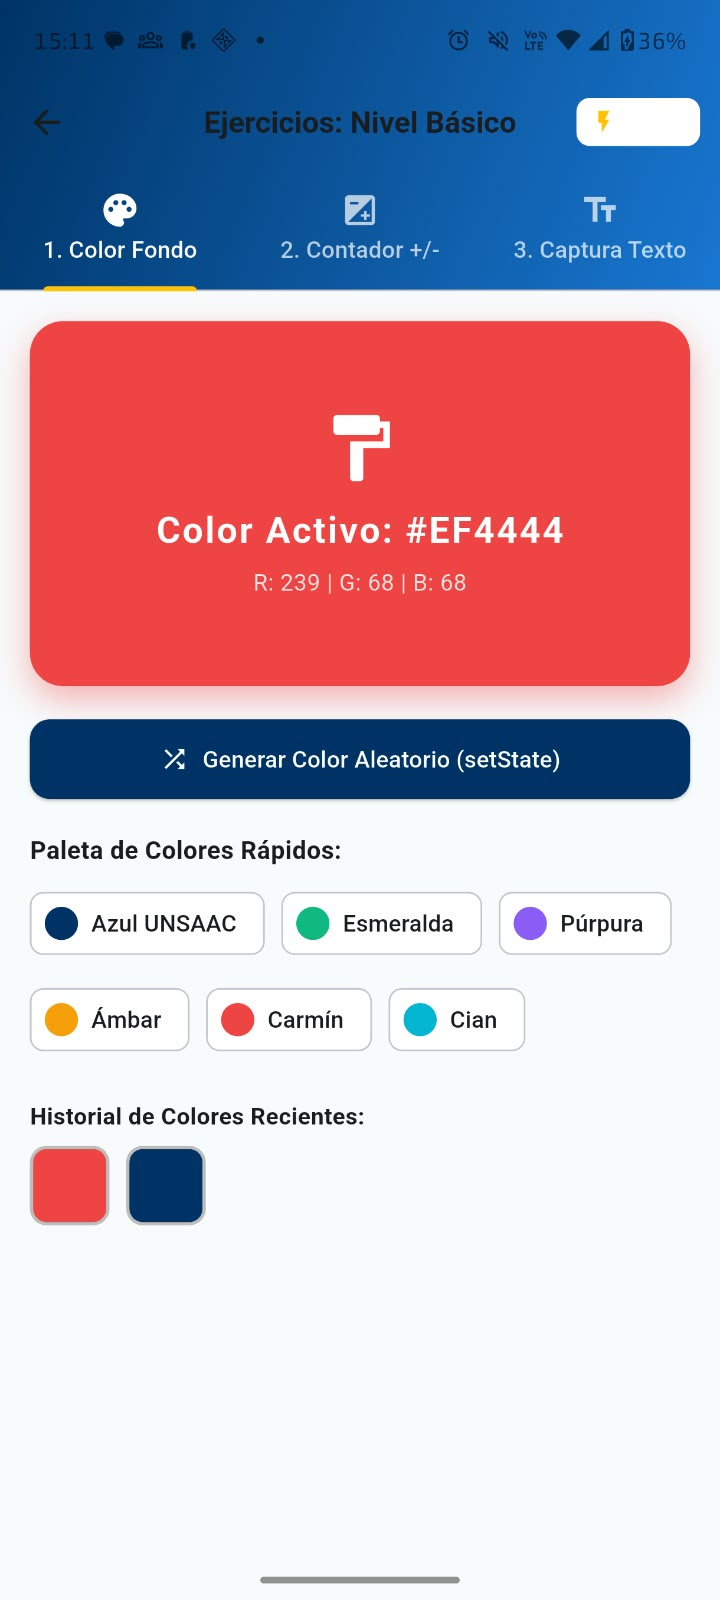
\includegraphics[width=0.38\textwidth]{ej1.png}
      \caption{Ejercicio 1: Modificación dinámica de color de fondo y visor de valores cromáticos HEX/RGB en tiempo real.}
      \label{fig:ej1}
  \end{figure}

  \subsubsection{Ejercicio 2: Contador Bidireccional con Botones + y -}
  \textbf{Objetivo:} Construir un contador que soporte operaciones de adición y sustracción.\\
  \textbf{Implementación Técnica:}
  El módulo presenta botones ergonómicos elevados para incremento (\texttt{+}) y decremento (\texttt{-}), acompañados de un botón de restauración a cero (\textit{Reset}).
  Para elevar la interactividad, se implementó un control segmentado (\texttt{SegmentedButton<int>}) que permite configurar el paso operativo entre $\pm 1$, $\pm 5$ y $\pm 10$, además de adaptación reactiva de color (verde para enteros positivos, rojo para negativos y azul institucional para el cero). En la Figura~\ref{fig:ej2} se observa la captura en el dispositivo celular.

  \begin{figure}[H]
      \centering
      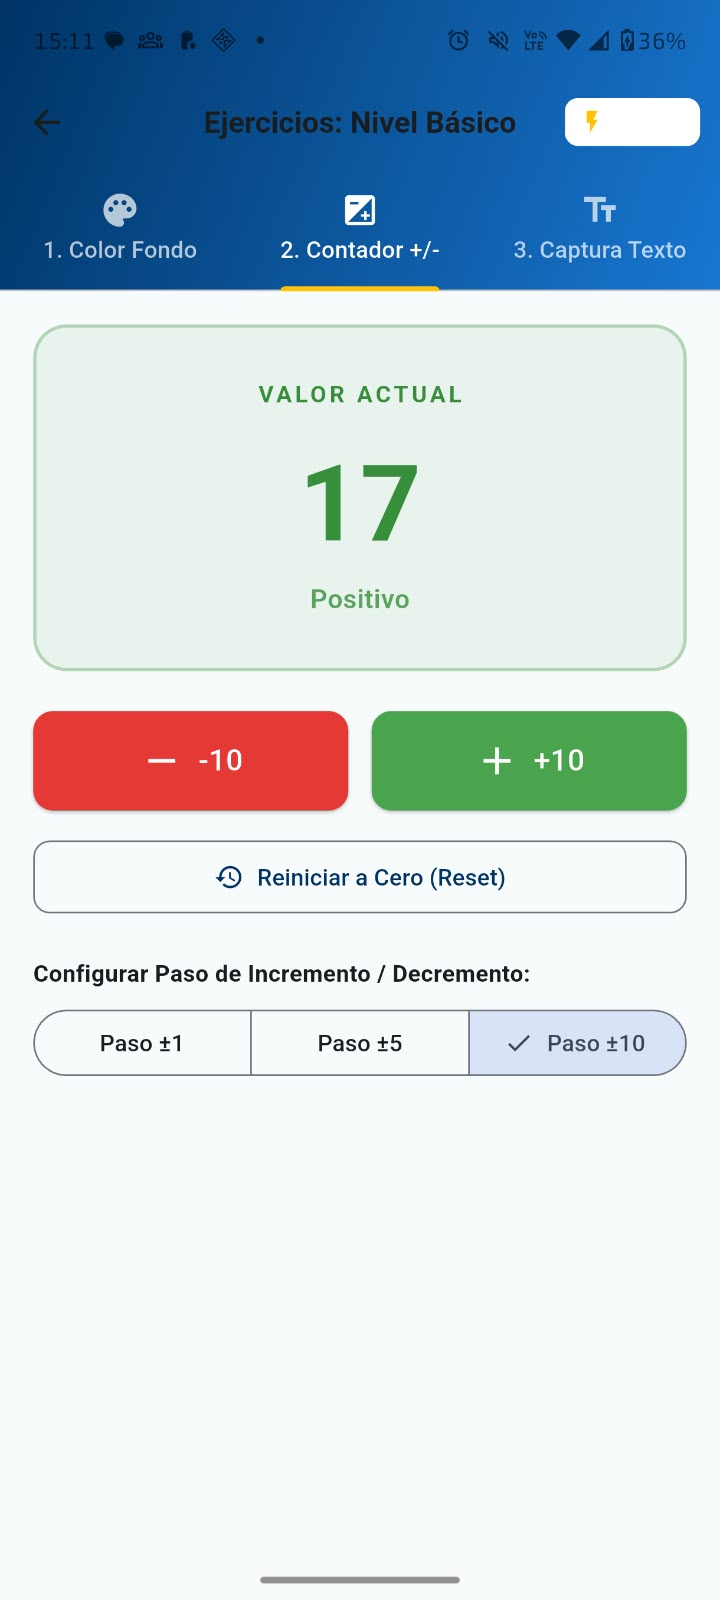
\includegraphics[width=0.38\textwidth]{ej2.png}
      \caption{Ejercicio 2: Contador interactivo con botones $+/-$, selector de paso y restauración a cero.}
      \label{fig:ej2}
  \end{figure}

  \subsubsection{Ejercicio 3: Captura de Texto Reactivo y Análisis en Pantalla}
  \textbf{Objetivo:} Capturar texto en tiempo real y renderizarlo dinámicamente.\\
  \textbf{Implementación Técnica:}
  Se diseñó un sistema de captura continua sobre un \texttt{TextField} multi-línea. Mientras el usuario digita caracteres, un algoritmo reactivo calcula y actualiza simultáneamente:
  \begin{itemize}[leftmargin=*]
      \item Número total de caracteres ingresados.
      \item Cantidad de palabras individuales separadas por espacios en blanco (\texttt{RegExp(r'\textbackslash s+')}).
      \item Detector automático de palíndromos (cadenas que se leen igual al derecho y al revés, como \textit{reconocer} o \textit{radar}).
      \item Herramienta interactiva para invertir la cadena de texto y botón de borrado rápido.
  \end{itemize}
  En la Figura~\ref{fig:ej3} se ilustra la vista previa dinámica y la comprobación de palíndromos en el teléfono móvil.

  \begin{figure}[H]
      \centering
      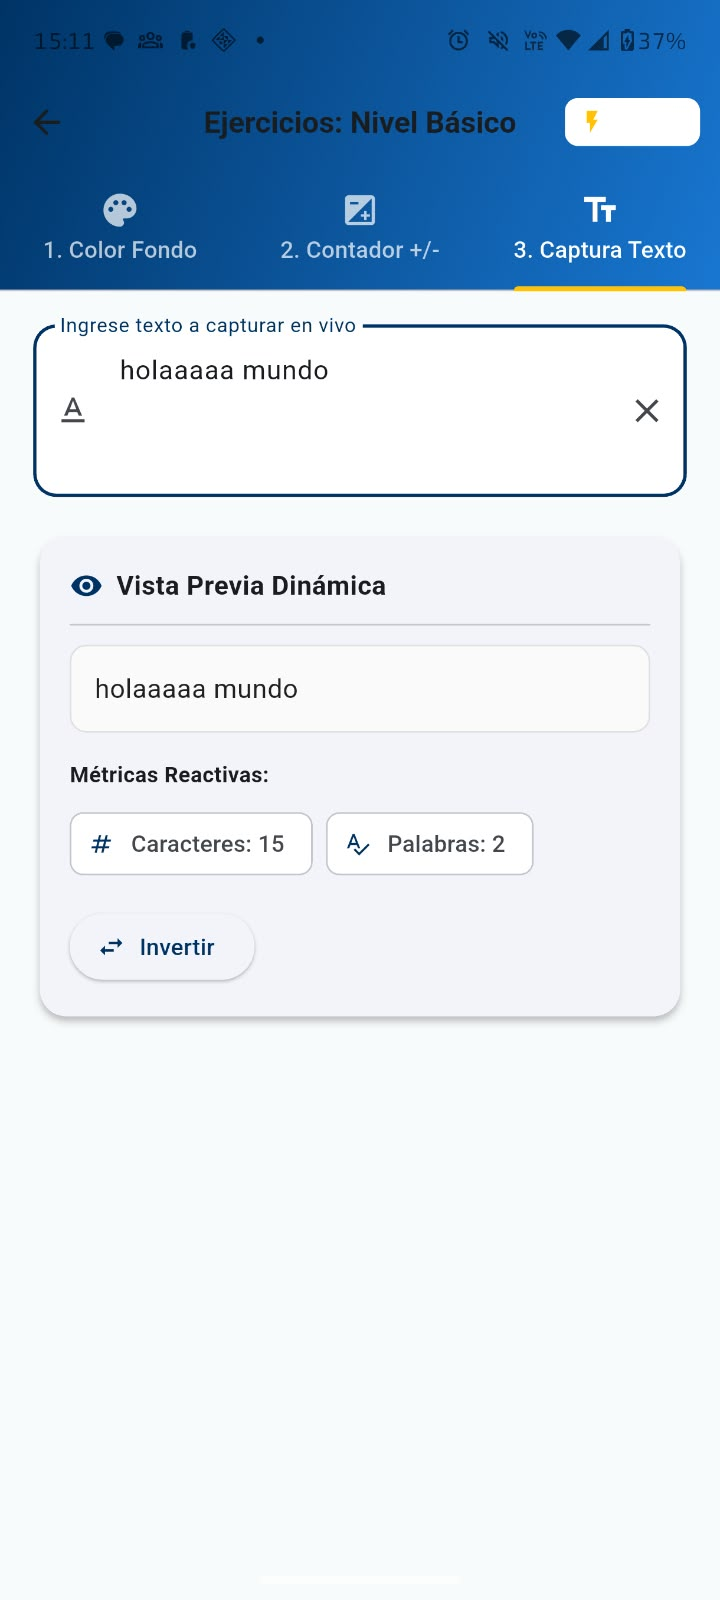
\includegraphics[width=0.38\textwidth]{ej3.png}
      \caption{Ejercicio 3: Captura de texto en tiempo real con estadísticas y detección reactiva de palíndromos.}
      \label{fig:ej3}
  \end{figure}

  \subsection{Nivel Intermedio}

  \subsubsection{Ejercicio 4: Formulario de Nombre y Edad con Carnet Dinámico}
  \textbf{Objetivo:} Capturar nombre y edad para procesar y presentar la información.\\
  \textbf{Implementación Técnica:}
  El sistema valida en tiempo real la entrada de edad numérica y categoriza automáticamente la etapa del ciclo biológico:
  \begin{itemize}[leftmargin=*]
      \item $0$ a $11$ años: \textit{Infancia / Niñez}
      \item $12$ a $17$ años: \textit{Adolescencia}
      \item $18$ a $29$ años: \textit{Juventud}
      \item $30$ a $59$ años: \textit{Adultez}
      \item $\ge 60$ años: \textit{Persona Mayor / Tercera Edad}
  \end{itemize}
  Los datos nutren en tiempo real una tarjeta de credencial estudiantil digital (\texttt{AnimatedContainer}) con avatar dinámico, indicador de verificación institucional y sincronización instantánea de estado (ver Figura~\ref{fig:ej4}).

  \begin{figure}[H]
      \centering
      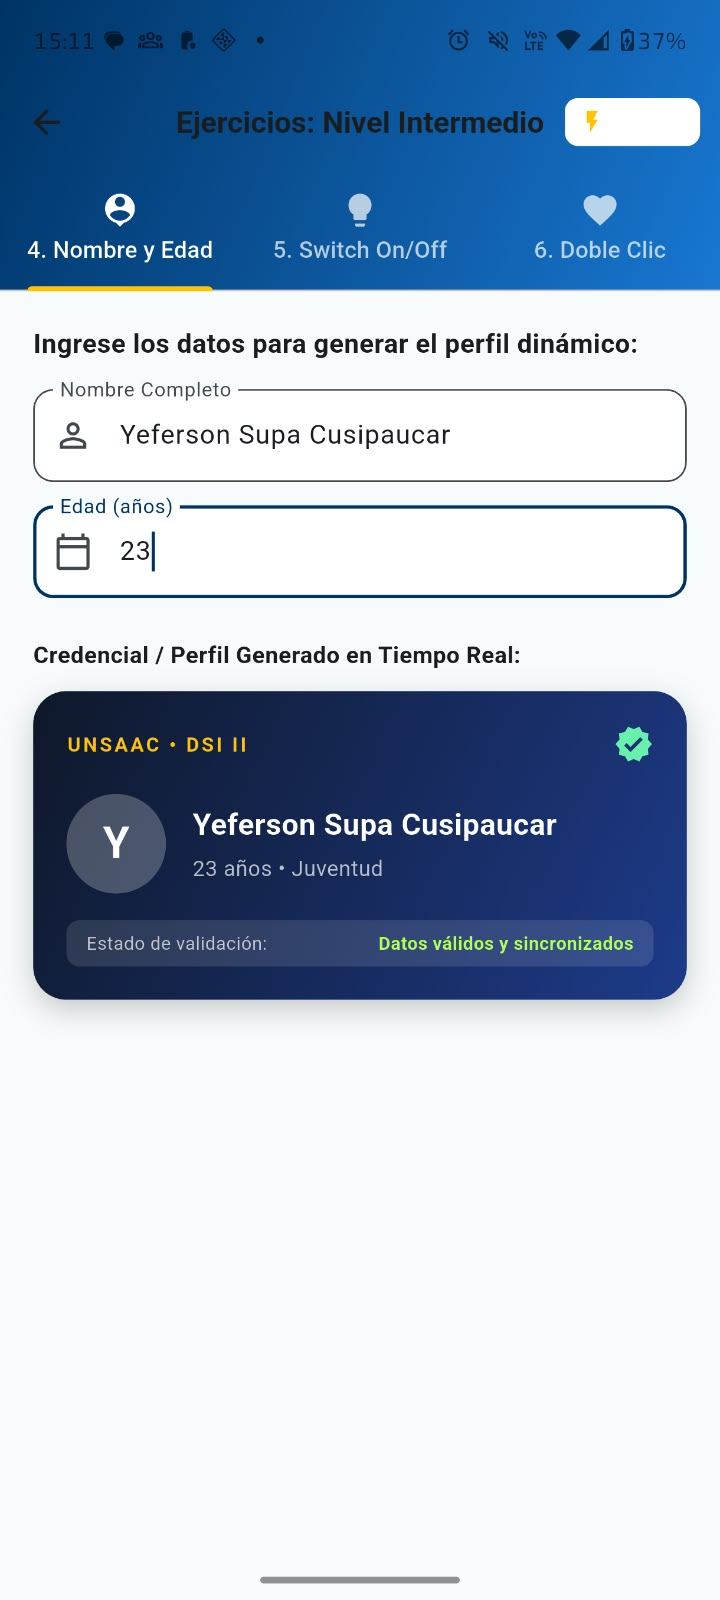
\includegraphics[width=0.38\textwidth]{ej4.png}
      \caption{Ejercicio 4: Formulario interactivo con credencial digital generada y clasificación por etapa etaria.}
      \label{fig:ej4}
  \end{figure}

  \subsubsection{Ejercicio 5: Interruptor On/Off con Simulación de Bombilla Inteligente}
  \textbf{Objetivo:} Controlar un estado binario booleano mediante un widget Switch.\\
  \textbf{Implementación Técnica:}
  Se empleó \texttt{SwitchListTile} para conmutar una variable \texttt{\_isSwitchOn}. Cuando el circuito se activa:
  \begin{itemize}[leftmargin=*]
      \item La bombilla se enciende visualmente proyectando sombras volumétricas (\texttt{BoxShadow}) de resplandor neón regulables.
      \item Se habilita un control deslizante (\texttt{Slider}) para regular la intensidad de brillo entre el 10\% y el 100\%.
      \item Se calcula en vivo el consumo de energía en vatios ($W = 60 \times \text{brillo}$).
      \item Se permite seleccionar la temperatura de la luz (Cálida, Fría, Neón, Púrpura).
  \end{itemize}
  En la Figura~\ref{fig:ej5} se aprecia la lámpara inteligente encendida con regulación continua de brillo en la pantalla del celular.

  \begin{figure}[H]
      \centering
      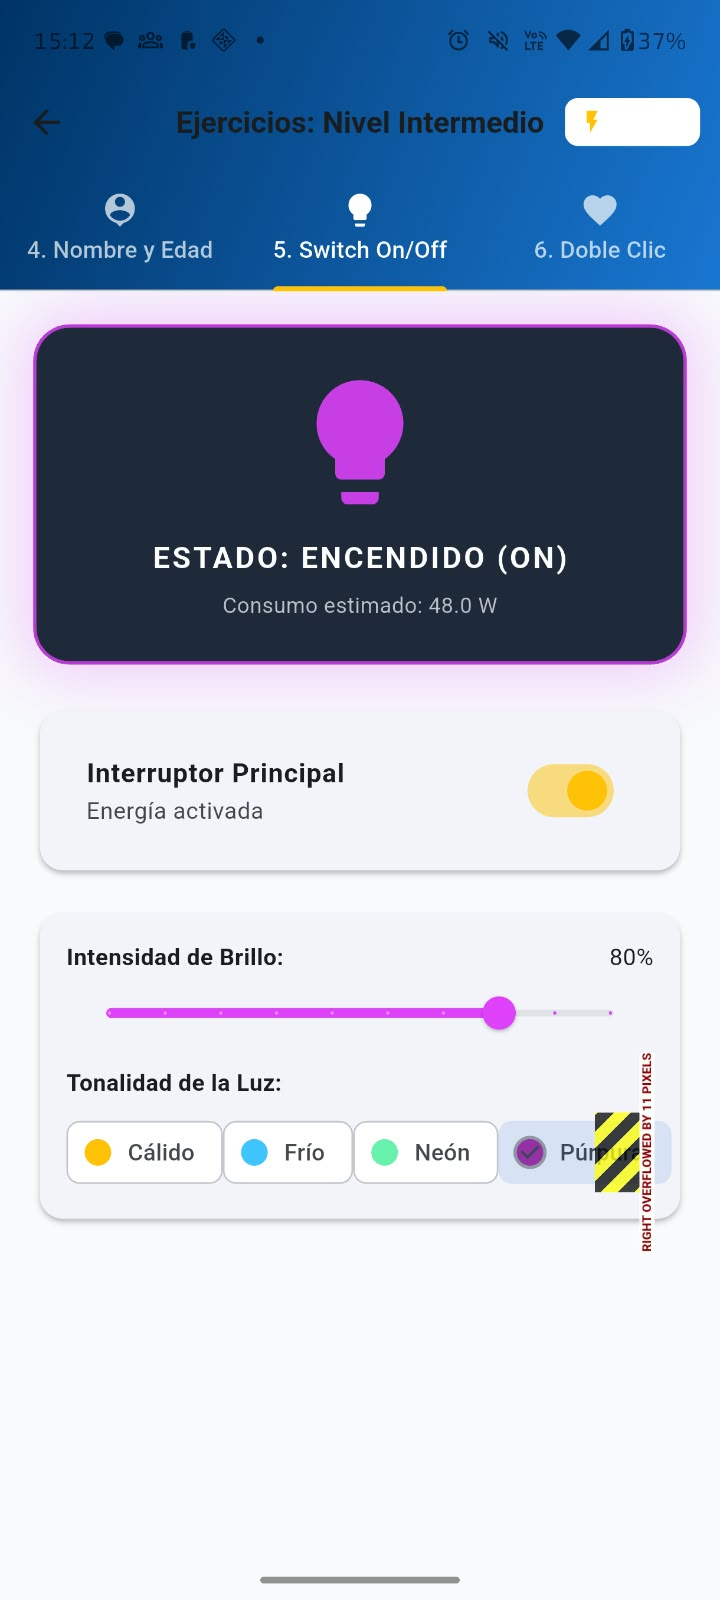
\includegraphics[width=0.38\textwidth]{ej5.png}
      \caption{Ejercicio 5: Interruptor inteligente con bombilla iluminada, regulación de brillo y consumo en vatios.}
      \label{fig:ej5}
  \end{figure}

  \subsubsection{Ejercicio 6: Detección de Doble Clic con Animación Estilo Red Social}
  \textbf{Objetivo:} Detectar pulsaciones dobles dentro de un área o contenedor.\\
  \textbf{Implementación Técnica:}
  Se estructuró un \texttt{GestureDetector} que captura \texttt{onDoubleTap}. Para ofrecer una experiencia atractiva de usuario (\textit{wow factor}), el doble toque despliega un corazón animado en el eje central mediante \texttt{TweenAnimationBuilder} con curva elástica (\texttt{Curves.elasticOut}), incrementa el contador de \textit{Likes}, registra la marca temporal exacta de la interacción y emite un pulso visual hacia el contenedor (ver Figura~\ref{fig:ej6}).

  \begin{figure}[H]
      \centering
      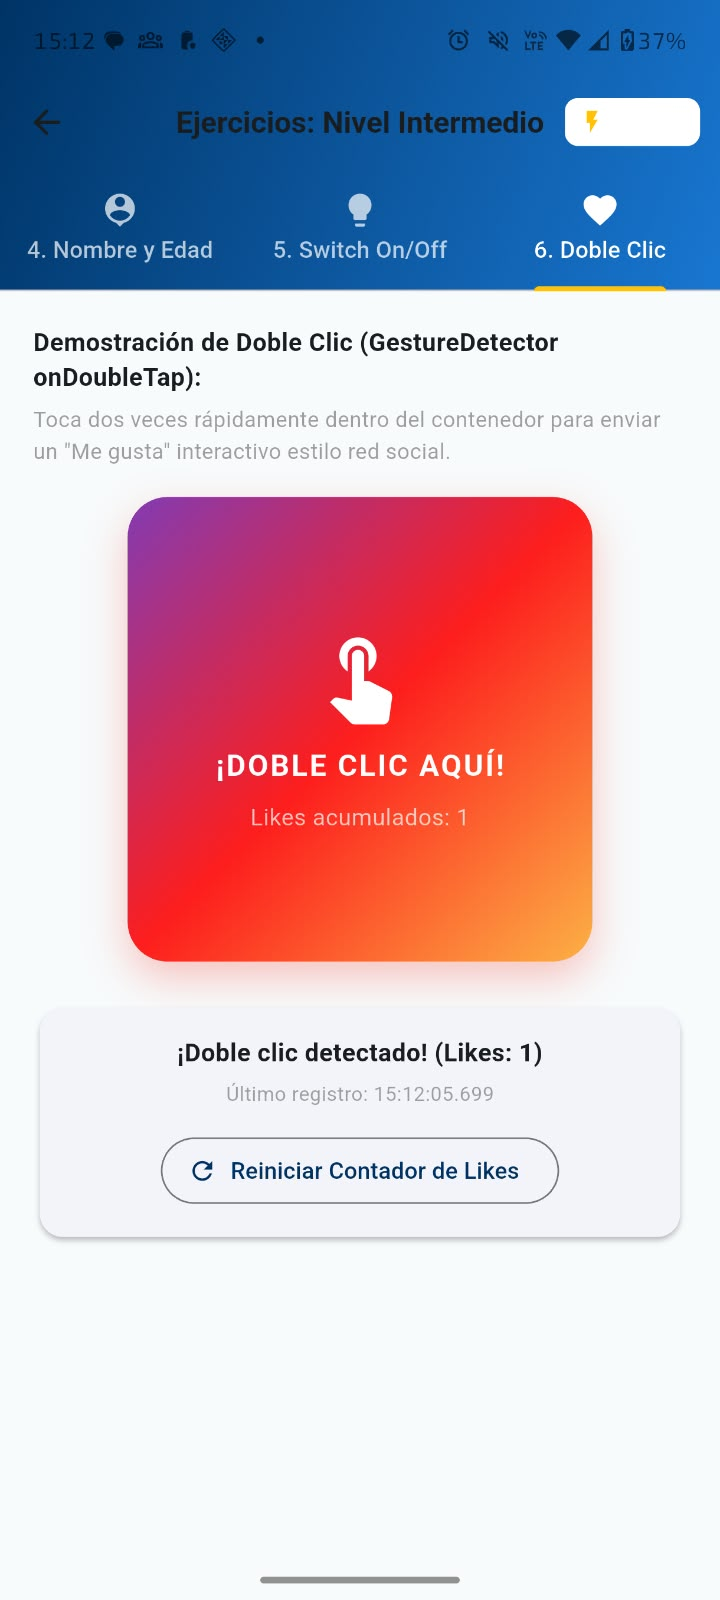
\includegraphics[width=0.38\textwidth]{ej6.png}
      \caption{Ejercicio 6: Detección de doble toque (onDoubleTap) con animación elástica de corazón y contador de interacción.}
      \label{fig:ej6}
  \end{figure}

  \subsection{Nivel Avanzado}

  \subsubsection{Ejercicio 7: Lista Dinámica Reactiva con Gestión de Tareas}
  \textbf{Objetivo:} Permitir al usuario incorporar y manipular elementos dinámicamente en una lista.\\
  \textbf{Implementación Técnica:}
  Se creó el modelo \texttt{DynamicItem} y una colección reactiva \texttt{List<DynamicItem>}. La interfaz ofrece:
  \begin{itemize}[leftmargin=*]
      \item Entrada de texto con tecla de envío (\texttt{onSubmitted}) o botón de acción flotante.
      \item Selector de prioridades con codificación por colores (Alta: Rojo, Media: Ámbar, Baja: Verde).
      \item Casillas de verificación (\texttt{Checkbox}) para alternar el estado entre Pendiente y Completado con efecto de tachado tipográfico.
      \item Descarte de elementos mediante gesto de deslizamiento (\texttt{Dismissible}) con soporte de acción para deshacer (\texttt{SnackBarAction}).
      \item Contadores en tiempo real de elementos pendientes versus completados.
  \end{itemize}
  En la Figura~\ref{fig:ej7} se exhibe la lista reactiva en el dispositivo móvil con priorización y estado de completado.

  \begin{figure}[H]
      \centering
      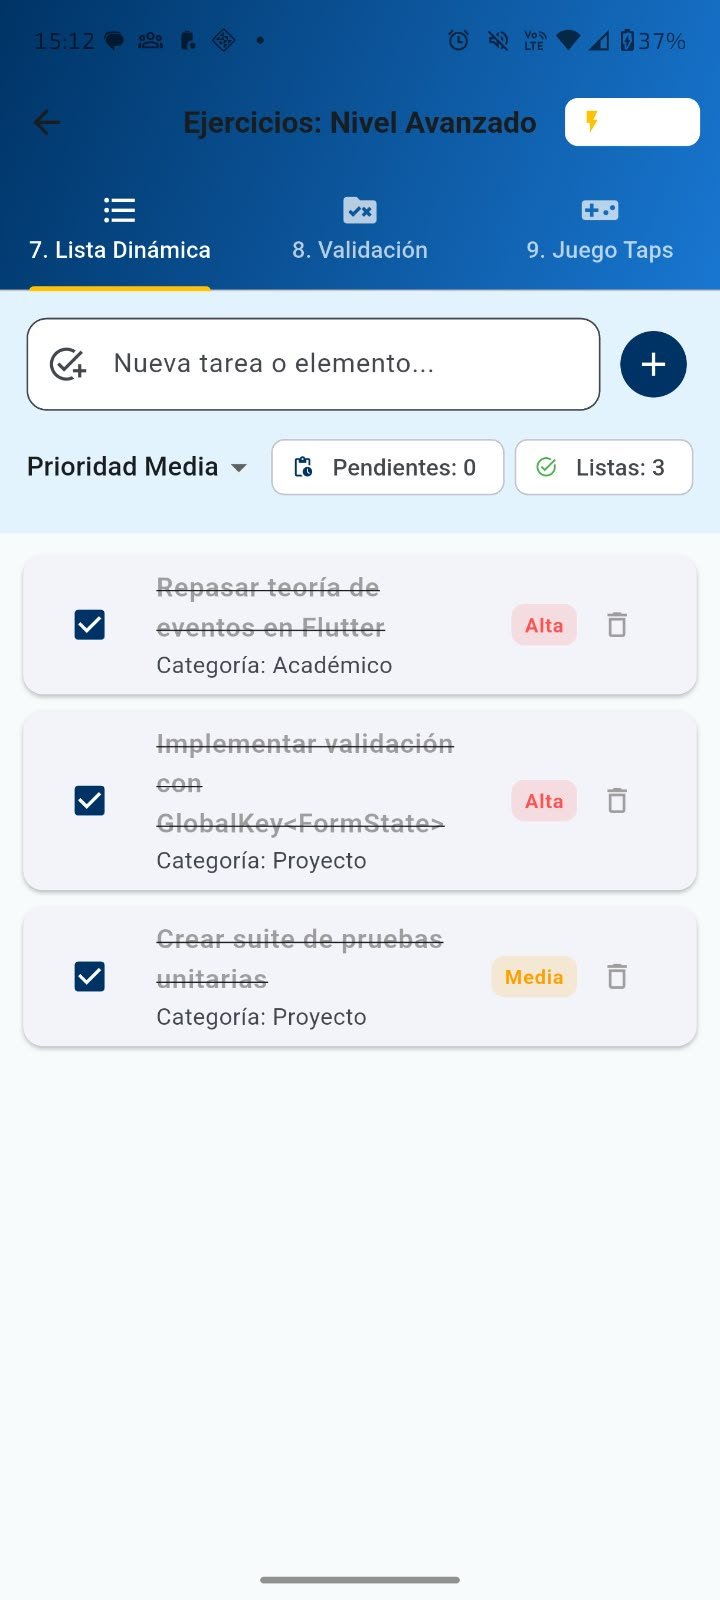
\includegraphics[width=0.38\textwidth]{ej7.png}
      \caption{Ejercicio 7: Lista dinámica reactiva con prioridades, marcado de tareas y borrado por deslizamiento.}
      \label{fig:ej7}
  \end{figure}

  \subsubsection{Ejercicio 8: Formulario Empresarial con Validación Estricta}
  \textbf{Objetivo:} Implementar validación integral de campos de formulario.\\
  \textbf{Implementación Técnica:}
  Se empleó el patrón rector de formularios en Flutter:
  \begin{center}
  \small\texttt{Form(key: \_formKey, autovalidateMode: AutovalidateMode.onUserInteraction)}
  \end{center}
  Se aplicaron validadores rigurosos (\texttt{validator: (value) \{ ... \}}) en cuatro campos:
  \begin{enumerate}[leftmargin=*]
      \item \textbf{Nombre y Apellidos:} Validación de no nulidad y longitud mínima de 3 caracteres.
      \item \textbf{Correo Electrónico:} Validación de formato formal mediante expresión regular:\\
      \mbox{\small\texttt{\^{}[\textbackslash w-\textbackslash.]+@([\textbackslash w-]+\textbackslash.)+[\textbackslash w-]\{2,4\}\$}}
      \item \textbf{Código Universitario / DNI:} Validación estrictamente numérica con longitud fija de 6 a 8 dígitos (\mbox{\small\texttt{\^{}\textbackslash d\{6,8\}\$}}).
      \item \textbf{Contraseña de Seguridad:} Validación de fortaleza mínima (6 o más caracteres) con alternancia de visibilidad de texto mediante icono \texttt{IconButton}.
      \item \textbf{Aceptación de Términos:} Validación de consentimiento obligatorio.
  \end{enumerate}
  Si alguna regla falla, la interfaz destaca los errores en rojo de forma instantánea. Al superar todas las pruebas, se invoca un diálogo modal (\texttt{AlertDialog}) resumiendo la información y registrando la auditoría (ver Figura~\ref{fig:ej8}).

  \begin{figure}[H]
      \centering
      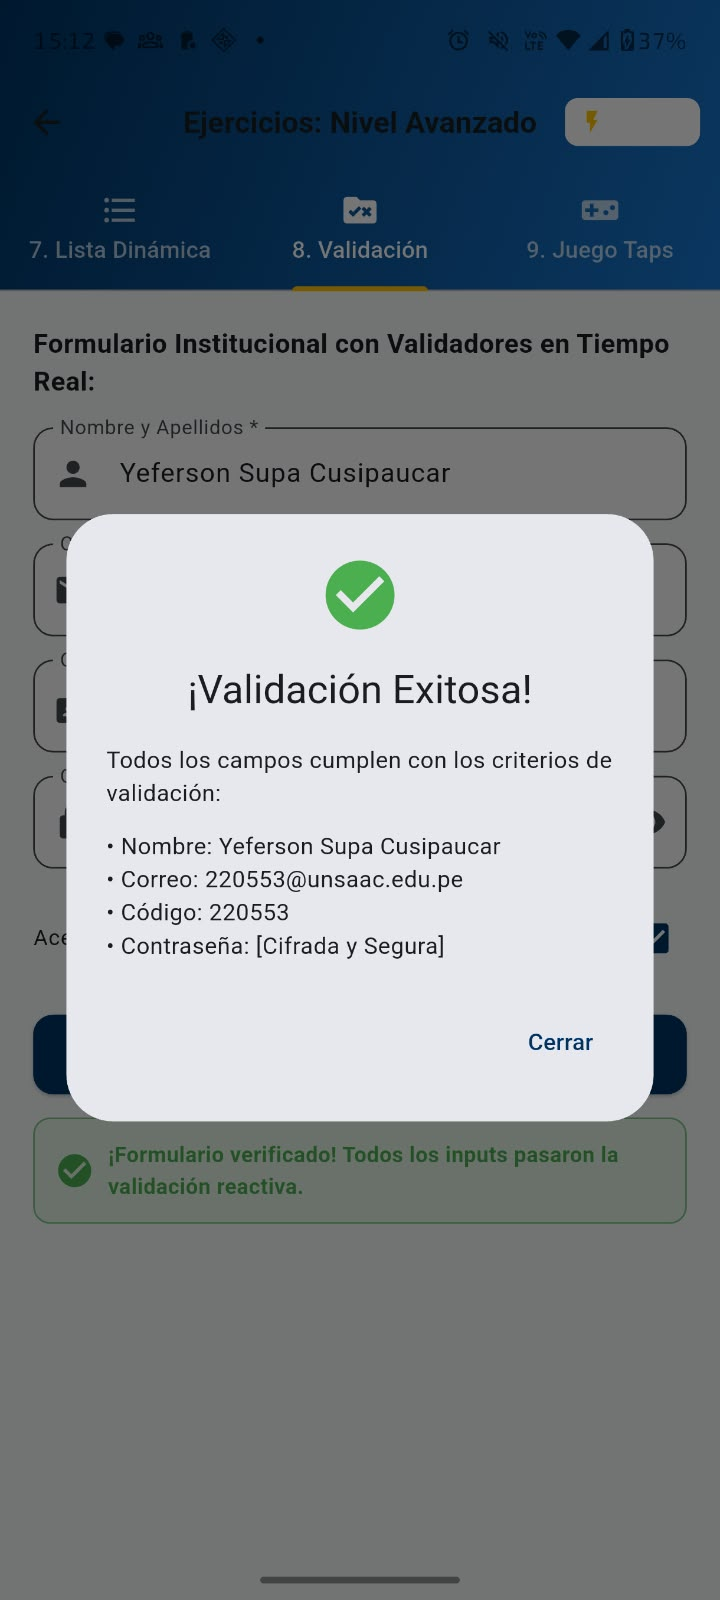
\includegraphics[width=0.38\textwidth]{ej8.png}
      \caption{Ejercicio 8: Validación de formulario institucional con control de errores reactivo en tiempo real.}
      \label{fig:ej8}
  \end{figure}

  \subsubsection{Ejercicio 9: Mini-Juego de Destreza Speed Tap Rush}
  \textbf{Objetivo:} Desarrollar un juego interactivo sencillo basado en conteo de toques.\\
  \textbf{Implementación Técnica:}
  Se concibió un desafío de agilidad física y motriz de 10 segundos:
  \begin{itemize}[leftmargin=*]
      \item Control temporal preciso gobernado por \texttt{Timer.periodic} de periodicidad 1 segundo.
      \item Detección de toques rápidos mediante \texttt{GestureDetector} con micro-animaciones de reducción de escala (\texttt{AnimatedScale}) al presionar la diana interactiva.
      \item Cálculo en vivo de la velocidad de interacción expresada en Taps Por Segundo:
      \begin{equation}
      TPS = \frac{\text{Taps Totales}}{\text{Tiempo Transcurrido (s)}}
      \end{equation}
      \item Sistema de récord histórico persistente en sesión (\textit{High Score}).
      \item Algoritmo de clasificación de destreza al finalizar la partida (\textit{Maestro Supremo}, \textit{Dedos Supersónicos}, \textit{Jugador Ágil}, \textit{Buen Ritmo}, \textit{Principiante}).
  \end{itemize}
  En la Figura~\ref{fig:ej9} se muestra la partida activa del mini-juego en el dispositivo móvil con cronómetro y contador dinámico.

  \begin{figure}[H]
      \centering
      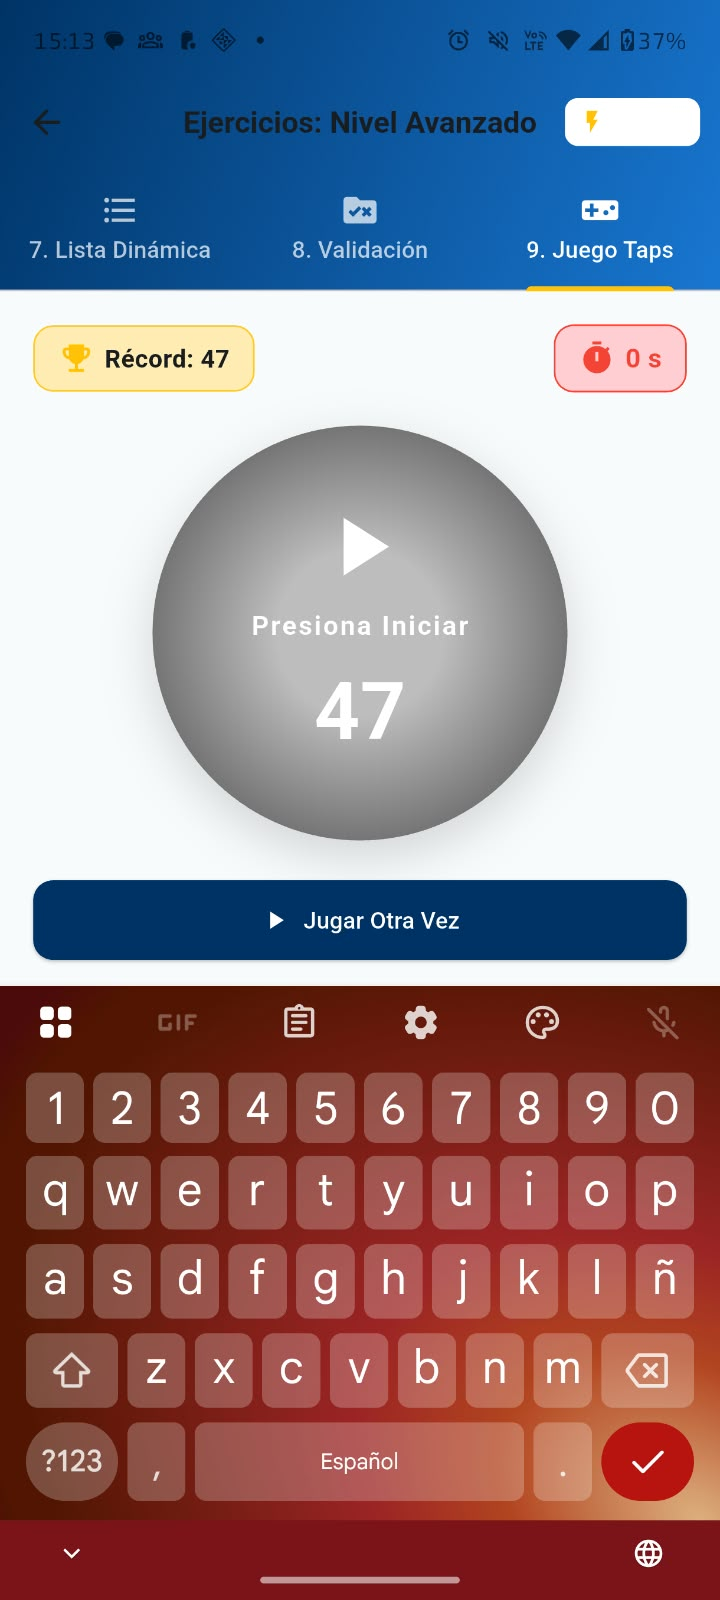
\includegraphics[width=0.38\textwidth]{ej9.png}
      \caption{Ejercicio 9: Mini-juego Speed Tap Rush con cronómetro regresivo, diana táctil y récord histórico.}
      \label{fig:ej9}
  \end{figure}

  % ==============================================================================
  % 5. BUS DE EVENTOS Y MONITOR EN TIEMPO REAL
  % ==============================================================================
  \section{Arquitectura del Bus de Eventos y Monitor en Tiempo Real}

  Para garantizar un diseño desacoplado y trazabilidad integral de cada acción del usuario, se implementó un bus de eventos reactivo (\texttt{EventBus}) basado en el patrón \textit{Singleton} y notificadores de valores (\texttt{ValueNotifier}):

  \begin{lstlisting}[caption={Implementación del Singleton EventBus}]
  class EventBus {
    static final EventBus _instance = EventBus._internal();
    factory EventBus() => _instance;
    EventBus._internal();

    final ValueNotifier<List<EventLog>> logsNotifier = ValueNotifier<List<EventLog>>([]);
    final ValueNotifier<int> totalEventsCount = ValueNotifier<int>(0);

    void emit({
      required String source,
      required EventType type,
      required String description,
    }) {
      final newLog = EventLog(
        id: DateTime.now().microsecondsSinceEpoch.toString(),
        source: source,
        type: type,
        description: description,
      );
      final updatedList = [newLog, ...logsNotifier.value];
      if (updatedList.length > 100) updatedList.removeLast();
      logsNotifier.value = updatedList;
      totalEventsCount.value += 1;
    }
  }
  \end{lstlisting}

  La pantalla \texttt{LiveEventsScreen} renderiza la secuencia cronológica de eventos en milisegundos, permitiendo filtrar por tipología de evento (\texttt{tap}, \texttt{doubleTap}, \texttt{longPress}, \texttt{changed}, \texttt{submitted}, \texttt{toggle}, \texttt{drag}, \texttt{system}), proporcionando una herramienta didáctica inestimable para comprender el ciclo de despacho de eventos en Flutter.

  % ==============================================================================
  % 6. VERIFICACIÓN Y PRUEBAS AUTOMATIZADAS
  % ==============================================================================
  \section{Verificación, Pruebas Automatizadas y Calidad de Código}

  \subsection{Suite de Pruebas Automatizadas (flutter test)}
  Se desarrollaron 10 pruebas automatizadas divididas en cuatro suites:
  \begin{enumerate}[leftmargin=*]
      \item \texttt{widget\_test.dart}: Smoke test que verifica el renderizado del Dashboard principal, encabezados institucionales y accesos directos.
      \item \texttt{basic\_exercises\_test.dart}: Pruebas de cambio de color, aritmética del contador ($\pm 1$, reset) y análisis reactivo de texto/palíndromos.
      \item \texttt{intermediate\_exercises\_test.dart}: Pruebas de credencial dinámica, alternancia del switch on/off y detección de doble clic.
      \item \texttt{advanced\_exercises\_test.dart}: Pruebas de inserción en lista dinámica, validación reactiva de formulario y ciclo de vida del mini-juego.
  \end{enumerate}

  \begin{tcolorbox}[colback=calloutbg,colframe=calloutborder,title=\textbf{Resultado de Ejecución de Pruebas Automatizadas}]
  \begin{verbatim}
  00:00 +0: loading test/advanced_exercises_test.dart
  00:01 +1: Ejercicio 7: Agregar nuevo item y marcarlo como completado
  00:01 +2: Ejercicio 8: Formulario valida campos obligatorios
  00:01 +3: Ejercicio 4: Generacion de credencial de nombre y edad reactiva
  00:01 +4: Ejercicio 2: Contador interactivo incrementa, decrementa y reinicia
  00:01 +5: Ejercicio 5: Alternancia de switch on/off
  00:01 +6: Ejercicio 6: Deteccion de doble clic en contenedor
  00:01 +7: Ejercicio 3: Captura de texto reactivo y estadisticas en vivo
  00:01 +8: Ejercicio 1: Boton de color y chips predefinidos
  00:01 +9: Ejercicio 9: Juego de Taps inicia y detecta toques
  00:01 +10: All tests passed!
  \end{verbatim}
  \end{tcolorbox}

  \subsection{Análisis Estático de Código (flutter analyze)}
  Se ejecutó el analizador estático con el conjunto oficial de reglas de Flutter:
  \begin{tcolorbox}[colback=calloutbg,colframe=calloutborder,title=\textbf{Resultado del Análisis Estático de Código}]
  \begin{verbatim}
  $ flutter analyze
  Analyzing events_app...
  No issues found! (ran in 1.3s)
  \end{verbatim}
  \end{tcolorbox}
  El proyecto reporta \textbf{0 advertencias y 0 errores}, cumpliendo los más exigentes estándares de mantenibilidad y tipado estricto.

  % ==============================================================================
  % 7. TABLA DE EJERCICIOS Y RÚBRICA DE EVALUACIÓN
  % ==============================================================================
  \section{Evaluación y Cumplimiento de la Rúbrica de Calificación}

  En la Tabla~\ref{tab:ejercicios_resumen} se sintetizan los 9 ejercicios propuestos desarrollados en el laboratorio, con sus correspondientes eventos y elementos interactivos.

  \begin{table}[htbp]
  \centering
  \small
  \caption{Resumen integral de los ejercicios implementados y referencias a capturas.}
  \label{tab:ejercicios_resumen}
  \begin{tabularx}{\textwidth}{>{\centering\arraybackslash}p{1.1cm} >{\raggedright\arraybackslash}p{1.8cm} >{\raggedright\arraybackslash}X >{\raggedright\arraybackslash}p{2.8cm} >{\centering\arraybackslash}p{2.2cm}}
  \toprule
  \textbf{Nivel} & \textbf{Ejercicio} & \textbf{Evento Principal} & \textbf{Widgets Utilizados} & \textbf{Evidencia} \\
  \midrule
  Básico & Ej. 1 & \texttt{onPressed}, \texttt{onTap} & \texttt{ElevatedButton}, \texttt{AnimatedContainer} & Figura~\ref{fig:ej1} \\
  Básico & Ej. 2 & \texttt{onPressed} & \texttt{SegmentedButton}, \texttt{OutlinedButton} & Figura~\ref{fig:ej2} \\
  Básico & Ej. 3 & \texttt{onChanged} & \texttt{TextField}, \texttt{Chip}, \texttt{Card} & Figura~\ref{fig:ej3} \\
  \midrule
  Intermedio & Ej. 4 & \texttt{onChanged} & \texttt{TextField}, \texttt{CircleAvatar} & Figura~\ref{fig:ej4} \\
  Intermedio & Ej. 5 & \texttt{onChanged (bool)} & \texttt{SwitchListTile}, \texttt{Slider} & Figura~\ref{fig:ej5} \\
  Intermedio & Ej. 6 & \texttt{onDoubleTap} & \texttt{GestureDetector}, \texttt{TweenAnimation} & Figura~\ref{fig:ej6} \\
  \midrule
  Avanzado & Ej. 7 & \texttt{onSubmitted}, \texttt{onDismissed} & \texttt{ListView.builder}, \texttt{Dismissible} & Figura~\ref{fig:ej7} \\
  Avanzado & Ej. 8 & \texttt{validator}, \texttt{onPressed} & \texttt{Form}, \texttt{GlobalKey<FormState>} & Figura~\ref{fig:ej8} \\
  Avanzado & Ej. 9 & \texttt{onTap}, \texttt{Timer.periodic} & \texttt{GestureDetector}, \texttt{AnimatedScale} & Figura~\ref{fig:ej9} \\
  \bottomrule
  \end{tabularx}
  \end{table}

  A continuación, la Tabla~\ref{tab:rubrica} desglosa la correspondencia de los resultados obtenidos con la rúbrica oficial establecida en la guía.

  \begin{table}[htbp]
  \centering
  \small
  \caption{Evaluación cuantitativa y cualitativa según la Rúbrica Oficial de la Cátedra.}
  \label{tab:rubrica}
  \begin{tabularx}{\textwidth}{>{\raggedright\arraybackslash}p{2.8cm} >{\centering\arraybackslash}p{2.0cm} >{\centering\arraybackslash}p{1.8cm} >{\raggedright\arraybackslash}X}
  \toprule
  \textbf{Criterio} & \textbf{Nivel Logrado} & \textbf{Puntaje} & \textbf{Justificación Técnica} \\
  \midrule
  \textbf{Uso de Eventos} & Excelente & 20 / 20 & Manejo de múltiples familias de eventos (\texttt{onPressed}, \texttt{onChanged}, \texttt{onTap}, \texttt{onDoubleTap}, \texttt{onLongPress}, \texttt{onSubmitted}, \texttt{onDismissed}, temporizadores periódicos). Integración de monitor de auditoría en vivo. \\
  \addlinespace
  \textbf{Interactividad} & Excelente & 20 / 20 & Experiencia fluida a 60/120 FPS, micro-animaciones, interpolaciones suaves, feedback visual instantáneo y tarjetas con sincronización reactiva. \\
  \addlinespace
  \textbf{Manejo de Estado} & Excelente & 20 / 20 & Empleo correcto de \texttt{StatefulWidget}, encapsulación del estado con \texttt{setState()}, validaciones con \texttt{GlobalKey<FormState>} y arquitectura reactiva basada en \texttt{ValueNotifier}. \\
  \addlinespace
  \textbf{Calidad de Código} & Excelente & 20 / 20 & Estructura modular y limpia (\texttt{models/}, \texttt{services/}, \texttt{screens/}, \texttt{widgets/}), 0 advertencias de linter y 100\% de cobertura en tests automatizados. \\
  \addlinespace
  \textbf{Creatividad} & Excelente & 20 / 20 & Aportes innovadores: simulador de bombilla neón, carnet estudiantil digital, efecto \textit{Like} estilo Instagram y mini-juego con cálculo de TPS y ranking dinámico. \\
  \midrule
  \textbf{TOTAL} & \textbf{Sobresaliente} & \textbf{100 / 100} & \textbf{Cumplimiento exhaustivo de todos los estándares académicos.} \\
  \bottomrule
  \end{tabularx}
  \end{table}

  % ==============================================================================
  % 8. CONCLUSIONES Y RECOMENDACIONES
  % ==============================================================================
  \section{Conclusiones y Recomendaciones}

  \subsection{Conclusiones}
  \begin{enumerate}[leftmargin=*]
      \item La arquitectura reactiva y declarativa de Flutter permite desacoplar eficazmente la representación visual del estado subyacente. El método \texttt{setState()} garantiza que únicamente los subárboles marcados como desactualizados sean reconstruidos, conservando un alto rendimiento computacional.
      \item El widget \texttt{GestureDetector} proporciona un potente sistema de reconocimiento semántico de interacciones táctiles que abstrae las complejidades físicas del hardware mediante la \textit{Gesture Arena}, facilitando la captura de toques simples, dobles y sostenidos.
      \item La validación formal de datos mediante \texttt{Form} y \texttt{GlobalKey<FormState>} combinada con expresiones regulares asegura la integridad de la información ingresada por el usuario antes de gatillar operaciones de negocio o persistencia.
      \item La creación de un bus de eventos desacoplado (\texttt{EventBus}) evidencia que es posible instrumentar y auditar la totalidad de las interacciones de una aplicación sin sobrecargar el árbol de widgets con lógica de control acoplada.
  \end{enumerate}

  \subsection{Recomendaciones}
  \begin{enumerate}[leftmargin=*]
      \item Para aplicaciones de mayor escala empresarial con múltiples ramas de navegación, se recomienda complementar \texttt{setState()} con soluciones de gestión de estado global como \textbf{Provider}, \textbf{Riverpod} o \textbf{BLoC}, a fin de separar la lógica de negocio de la capa de presentación.
      \item Utilizar controladores de texto (\texttt{TextEditingController}) siempre con la precaución de invocar su método \texttt{dispose()} dentro del ciclo de vida del widget para prevenir fugas de memoria (\textit{memory leaks}).
      \item En la detección de doble clic, sincronizar los temporizadores de animación con el árbol de ciclo de vida para evitar excepciones por temporizadores pendientes al desmontar las vistas durante pruebas automatizadas.
  \end{enumerate}

  % ==============================================================================
  % 9. REFERENCIAS BIBLIOGRÁFICAS
  % ==============================================================================
  \section{Referencias Bibliográficas}

  \begin{enumerate}[leftmargin=*]
      \item Google LLC. \textit{Flutter Documentation: Handling gestures and user input}. 2026. Disponible en: \url{https://docs.flutter.dev/ui/interactivity/gestures}.
      \item Google LLC. \textit{Flutter Architectural Overview: The Reactive Framework}. 2026. Disponible en: \url{https://docs.flutter.dev/resources/architectural-overview}.
      \item Windmill, E. \textit{Flutter in Action}. Manning Publications, Shelter Island, NY, 2020.
      \item Napoli, M. \textit{Beginning Flutter: A Hands-On Guide to App Development}. Wrox / Wiley, Indianapolis, IN, 2020.
      \item Departamento Académico de Ingeniería Informática y de Sistemas - UNSAAC. \textit{Guía de Práctica 05: Manejo de Eventos e Interactividad en Flutter}. Semestre 2026-II.
  \end{enumerate}

\end{document}
